\chapter{Aromaticidad y sustitución electrófila aromática}\label{ch:b2:aromatic-substitution}

El agua de bromo pierde su color en pocos segundos cuando se agita con un alqueno,
y no lo pierde en absoluto con el benceno. Sin embargo, el benceno sí reacciona con el bromo en cuanto se
añade un poco de bromuro de hierro(III), y el producto, el bromobenceno, conserva
su anillo \omterm{def:b2:huckel:aromatic}{aromático} de seis eslabones: se ha sustituido un hidrógeno, no se ha
adicionado nada. Los anillos \omterm{def:b2:huckel:aromatic}{aromáticos} se sustituyen en lugar de adicionarse, porque la adición
tiraría por la borda la estabilización calculada en el \cref{ch:b2:huckel}. El mismo
mecanismo nitra, sulfona, alquila y acila los anillos bencénicos, y
los grupos ya presentes en un anillo deciden, con una regularidad sorprendente, adónde va
el siguiente.

\begin{recall}
\Cref{ch:b2:huckel}: la aromaticidad y la \omterm{def:b2:huckel:delocalisation}{energía de deslocalización} del benceno. El volumen
del primer año: adiciones electrófilas a los alquenos, efectos inductivo y mesómero, grupos dadores y
aceptores, carbocationes y sus transposiciones, postulado de Hammond, ácidos de Lewis,
perfiles de energía.
\end{recall}

\begin{omfigure}
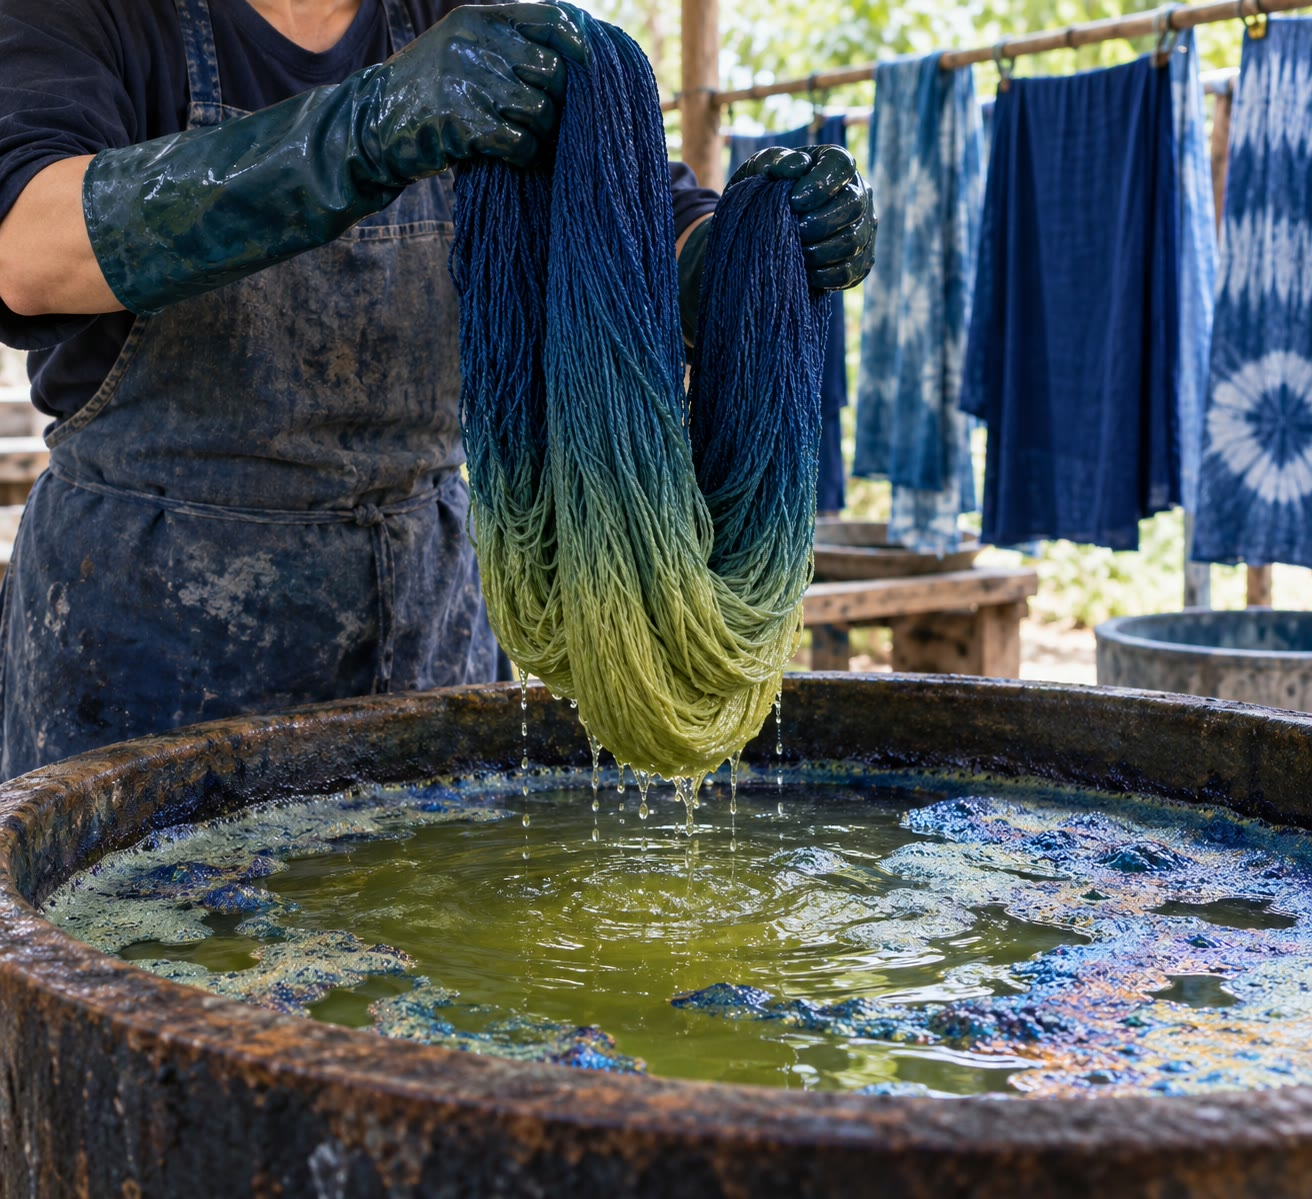
\includegraphics[width=0.55\linewidth]{images/book3/ai/b2-22-indigo-vat-2.jpg}

{\small Teñido de hilo en una cuba de índigo (ilustración). El hilo sale de la cuba amarillo verdoso, empapado
de la forma reducida y soluble del colorante, y se vuelve azul al aire, cuando el oxígeno la devuelve al
índigo insoluble. El índigo, como la mayoría de los colorantes, está construido sobre anillos \omterm{def:b2:huckel:aromatic}{aromáticos};
la industria de los colorantes del siglo XIX nació de las reacciones de sustitución de este
capítulo aplicadas al benceno del alquitrán de hulla.}
\end{omfigure}

\section{Sustitución, no adición}

\begin{definition}[Areno]\label{def:b2:aromatic-substitution:arene}
Un \emph{areno}\index{areno} es un hidrocarburo que contiene al menos un anillo \omterm{def:b2:huckel:aromatic}{aromático}, como el
benceno, el tolueno (metilbenceno) o el naftaleno; un grupo arilo (\ce{Ar}) es un areno al que le falta
un hidrógeno.
\end{definition}

\begin{proposition}[Por qué el benceno no se adiciona]\label{prop:b2:aromatic-substitution:no-addition}
Una adición al benceno convertiría el anillo \omterm{def:b2:huckel:aromatic}{aromático} en un ciclohexadieno no \omterm{def:b2:huckel:aromatic}{aromático} y
perdería la mayor parte de los \qty{150}{kJ/mol} de estabilización \omterm{def:b2:huckel:aromatic}{aromática}; la sustitución la conserva.
\end{proposition}

\begin{proof}[Argumento]
En el \cref{ch:b2:huckel} se halló que la hidrogenación del benceno a ciclohexa-1,3-dieno es
\omterm{def:b2:reaction-enthalpy:exothermic}{endotérmica} (\qty{+22}{kJ/mol}, a partir de \qty{-206.0}{} y \qty{-227.7}{kJ/mol}), mientras que la de un
doble enlace ordinario libera \qty{119}{kJ/mol}: la primera adición es la etapa costosa.
Tras la primera etapa electrófila, el catión formado puede adicionar un nucleófilo, lo que
deja un \omterm{def:b2:frontier-orbitals:diels-alder}{dieno} no \omterm{def:b2:huckel:aromatic}{aromático}, o perder un protón, lo que restaura el anillo \omterm{def:b2:huckel:aromatic}{aromático}. El segundo
camino es mucho más favorable.
% ledger: dfh:C6H6_g, dfh:C6H8_g, dfh:C6H10_g, dfh:C6H12_g
\end{proof}

\section{El mecanismo}

\begin{definition}[Sustitución electrófila aromática]\label{def:b2:aromatic-substitution:seAr}
Una \emph{sustitución electrófila aromática}\index{sustitucion electrofila aromatica@sustitución electrófila aromática}
sustituye un hidrógeno de un anillo \omterm{def:b2:huckel:aromatic}{aromático} por un electrófilo \ce{E+}. El electrófilo se
une primero a un carbono del anillo, dando un catión en el que ese carbono es tetraédrico y la
carga positiva se reparte sobre los otros cinco: el \emph{intermedio de Wheland}\index{intermedio de Wheland}
(un ion arenio). Una base retira después el protón del carbono tetraédrico.
\end{definition}

\begin{proposition}[Dos etapas]\label{prop:b2:aromatic-substitution:mechanism}
La primera etapa, que destruye la aromaticidad, es la lenta; la pérdida del protón,
que la restaura, es rápida.
\end{proposition}

\begin{proof}[Argumento]
El \omterm{def:b2:aromatic-substitution:seAr}{intermedio de Wheland} es un carbocatión estabilizado por deslocalización sobre tres carbonos,
pero no \omterm{def:b2:huckel:aromatic}{aromático}: está muy por encima de los reactivos y, por el postulado de Hammond, el
estado de transición que conduce a él se le parece en estructura y en energía. La segunda etapa
desciende hacia un producto \omterm{def:b2:huckel:aromatic}{aromático}: su barrera es baja.
\end{proof}

\begin{omfigure}
\begin{tikzpicture}
\begin{axis}[width=0.55\linewidth, height=5.4cm, xmin=-0.2, xmax=4.2, ymin=-5.5, ymax=11.5,
  axis x line=bottom, axis y line=left, xtick=\empty, ytick=\empty,
  xlabel={coordenada de reacción}, ylabel={energía}, label style={font=\small}, clip=false]
\addplot[omDef, thick] table[x=x, y=sub] {figdata/out/bachelor-2-aromatic-profile.dat};
\addplot[omThm, thick, dashed, restrict x to domain=2:4] table[x=x, y=add] {figdata/out/bachelor-2-aromatic-profile.dat};
\node[font=\scriptsize, anchor=north west] at (axis cs:0.0,-0.6) {\ce{ArH + E+}};
\node[font=\scriptsize, anchor=north] at (axis cs:2,5.7) {Wheland};
\node[font=\scriptsize, anchor=west, omDef] at (axis cs:4.05,-4.0) {\ce{ArE + H+}};
\node[font=\scriptsize, anchor=west, omThm] at (axis cs:4.05,2.0) {producto de adición};
\node[font=\scriptsize, anchor=south] at (axis cs:1,10.1) {lenta};
\end{axis}
\end{tikzpicture}

{\small Perfil de energía de una \omterm{def:b2:aromatic-substitution:seAr}{sustitución electrófila aromática}, esquema (un modelo).
La primera etapa, que forma el \omterm{def:b2:aromatic-substitution:seAr}{intermedio de Wheland}, tiene la barrera más alta. La pérdida de un
protón (trazo continuo) restaura el anillo \omterm{def:b2:huckel:aromatic}{aromático}; la adición de un nucleófilo (discontinuo) dejaría un
producto por encima de los reactivos.}
\end{omfigure}

\begin{omfigure}
\setchemfig{atom sep=2em}
\schemestart
\chemfig{HO-\chemabove{N}{\scriptstyle +}(=[1]O)-[7]\chemabove{O}{\scriptstyle -}} \+ \chemfig{H_2SO_4}
\arrow{<=>}
\chemfig{O=N^{+}=O} \+ \chemfig{HSO_4^{-}} \+ \chemfig{H_2O}
\schemestop

\medskip
\begin{tikzpicture}[font=\small, >={Stealth}]
\tikzset{pics/whel/.style n args={4}{code={
    \foreach \k in {0,...,5} \draw[thick] ({90+60*\k}:0.7) -- ({150+60*\k}:0.7);
    \foreach \k in {#1} \draw[thick] ($({90+60*\k}:0.56)!0.18!({150+60*\k}:0.56)$) -- ($({90+60*\k}:0.56)!0.82!({150+60*\k}:0.56)$);
    \ifnum#2>-1 \node[font=\scriptsize] at ({90+60*#2}:0.36) {$+$};\fi
    \draw[thick] (270:0.7) -- ++(-125:0.42) node[anchor=north east, inner sep=1pt, font=\scriptsize] {H};
    \draw[thick] (270:0.7) -- ++(-55:0.42) node[anchor=north west, inner sep=1pt, font=\scriptsize] {#4};
    \if\relax\detokenize{#3}\relax\else
      \draw[thick] (90:0.7) -- (90:1.1) node[anchor=south, inner sep=1pt, font=\scriptsize] {#3};\fi
  }}}
  \foreach \k in {0,...,5} \draw[thick] ({90+60*\k}:0.7) -- ({150+60*\k}:0.7);
  \foreach \k in {0,2,4} \draw[thick] ($({90+60*\k}:0.56)!0.18!({150+60*\k}:0.56)$) -- ($({90+60*\k}:0.56)!0.82!({150+60*\k}:0.56)$);
  \node at (1.3,0) {$+$};
  \node at (2.0,0) {\ce{NO2+}};
  \draw[->, thick] (2.6,0) -- (3.8,0) node[midway, above, font=\scriptsize] {lenta};
  \pic at (4.7,0.1) {whel={1,4}{0}{}{\ce{NO2}}};
  \draw[->, thick] (5.6,0) -- (6.8,0) node[midway, above, font=\scriptsize] {rápida} node[midway, below, font=\scriptsize] {$-$\ce{H+}};
  \begin{scope}[xshift=7.7cm]
    \foreach \k in {0,...,5} \draw[thick] ({90+60*\k}:0.7) -- ({150+60*\k}:0.7);
    \foreach \k in {0,2,4} \draw[thick] ($({90+60*\k}:0.56)!0.18!({150+60*\k}:0.56)$) -- ($({90+60*\k}:0.56)!0.82!({150+60*\k}:0.56)$);
    \draw[thick] (270:0.7) -- (270:1.1) node[anchor=north, font=\scriptsize] {\ce{NO2}};
  \end{scope}
\end{tikzpicture}
\par\vspace{6pt}

{\small Nitración del benceno. El ácido sulfúrico protona el ácido nítrico, que pierde agua: el
ion nitronio \ce{NO2+} es el electrófilo. Se une a un carbono (lenta), dando el
\omterm{def:b2:aromatic-substitution:seAr}{intermedio de Wheland}, cuya carga positiva se reparte por el anillo; la pérdida de un protón
(rápida) da nitrobenceno.}
\end{omfigure}

\section{Las reacciones}

\paragraph{Halogenación.} El bromo o el cloro solos son electrófilos demasiado débiles; un ácido de Lewis
(\ce{FeBr3}, \ce{AlCl3}) polariza el halógeno uniéndose a uno de sus átomos, y el bromo
externo ataca el anillo.

\paragraph{Nitración.} Una mezcla de ácidos nítrico y sulfúrico concentrados (arriba) da el
ion nitronio.

\paragraph{Sulfonación.} El ácido sulfúrico fumante (\ce{SO3} en \ce{H2SO4}) da ácido bencenosulfónico.
La reacción es reversible: calentar el ácido sulfónico en ácido acuoso diluido elimina de nuevo el
grupo \ce{SO3H}, lo que lo convierte en un útil grupo bloqueante temporal.

\begin{definition}[Reacciones de Friedel--Crafts]\label{def:b2:aromatic-substitution:friedel-crafts}
Una \emph{alquilación de Friedel--Crafts}\index{alquilacion de Friedel--Crafts@alquilación de Friedel--Crafts} une un grupo alquilo
a un anillo \omterm{def:b2:huckel:aromatic}{aromático} a partir de un halogenoalcano y un ácido de Lewis (\ce{AlCl3}). Una
\emph{acilación de Friedel--Crafts}\index{acilacion de Friedel--Crafts@acilación de Friedel--Crafts} une un grupo acilo
\ce{RCO} a partir de un cloruro de acilo y \ce{AlCl3}, a través del \emph{ion acilio}\index{ion acilio}
\ce{R-C#O+}, dando una aril cetona.
\end{definition}

\begin{proposition}[Límites de las reacciones de Friedel--Crafts]\label{prop:b2:aromatic-substitution:friedel-crafts-limits}
La \omterm{def:b2:aromatic-substitution:friedel-crafts}{alquilación de Friedel--Crafts} sufre transposiciones del carbocatión y
polialquilación; la acilación se detiene tras una sustitución, no da transposiciones y necesita al
menos un equivalente de \ce{AlCl3}. Ninguna de las dos funciona sobre un anillo que lleve un grupo fuertemente
desactivante.
\end{proposition}

\begin{proof}[Argumento]
El electrófilo alquilante es un carbocatión (o un complejo polarizado que se comporta como tal),
que se transpone a otro más estable por desplazamientos de hidruro o de alquilo: el 1-cloropropano da
sobre todo isopropilbenceno. Un grupo alquilo activa el anillo (sección siguiente), de modo que el producto
reacciona más deprisa que el benceno y vuelve a alquilarse. El \omterm{def:b2:aromatic-substitution:friedel-crafts}{ion acilio} está estabilizado por
resonancia (\ce{R-C+=O} $\leftrightarrow$ \ce{R-C#O+}) y no se transpone; el grupo acilo
desactiva el anillo, de modo que el producto no sigue reaccionando; y la cetona formada une
\ce{AlCl3} por su oxígeno, retirando el catalizador de la reacción: se consume un
equivalente. Un anillo fuertemente desactivado es un nucleófilo demasiado pobre para estos electrófilos débiles.
\end{proof}

\section{Efectos de los sustituyentes}

\begin{definition}[Grupos orientadores]\label{def:b2:aromatic-substitution:directing}
Un sustituyente de un anillo bencénico es un \emph{grupo activante}\index{grupo activante} si el
anillo reacciona más deprisa que el benceno, y un \emph{grupo desactivante}\index{grupo desactivante} si
reacciona más despacio. Es un \emph{orientador orto/para}\index{orientador orto/para} si el nuevo
grupo entra principalmente en las posiciones contiguas a él y en la opuesta, y un \emph{orientador
meta}\index{orientador meta} si entra principalmente en las posiciones separadas por un carbono.
\end{definition}

\begin{proposition}[Dadores y aceptores]\label{prop:b2:aromatic-substitution:directing}
Los grupos que ceden electrones al anillo por efecto mesómero (\ce{-OH}, \ce{-OCH3}, \ce{-NH2},
\ce{-NHCOCH3}) o por efecto inductivo e \omterm{def:b2:fragment-orbitals:hyperconjugation}{hiperconjugación} (alquilos) activan el anillo y orientan
a orto/para. Los grupos que atraen electrones por efecto mesómero (\ce{-NO2}, \ce{-CN}, \ce{-COR},
\ce{-COOH}, \ce{-SO3H}) lo desactivan y orientan a meta.
\end{proposition}

\begin{proof}
Compárense los \omterm{def:b2:aromatic-substitution:seAr}{intermedios de Wheland}. Para un ataque en orto o en para respecto a un sustituyente G, una de las
tres estructuras de resonancia pone la carga positiva sobre el carbono que lleva G; para un ataque en meta,
ninguna. Un G dador (un par no enlazante sobre O o N) estabiliza una carga positiva sobre el carbono al que
está unido, añadiendo una cuarta estructura de resonancia en la que todos los átomos tienen octeto: los intermedios orto
y para descienden y, por el postulado de Hammond, también los estados de transición
que conducen a ellos. Un G aceptor desestabiliza una carga positiva sobre su carbono: los intermedios orto y para
suben, y el ataque en meta, que evita esa estructura, es el menos
desfavorecido, aunque más lento que sobre el benceno.
\end{proof}

\begin{omfigure}
\begin{tikzpicture}[font=\small]
\tikzset{pics/whel/.style n args={4}{code={
    \foreach \k in {0,...,5} \draw[thick] ({90+60*\k}:0.7) -- ({150+60*\k}:0.7);
    \foreach \k in {#1} \draw[thick] ($({90+60*\k}:0.56)!0.18!({150+60*\k}:0.56)$) -- ($({90+60*\k}:0.56)!0.82!({150+60*\k}:0.56)$);
    \ifnum#2>-1 \node[font=\scriptsize] at ({90+60*#2}:0.36) {$+$};\fi
    \draw[thick] (270:0.7) -- ++(-125:0.42) node[anchor=north east, inner sep=1pt, font=\scriptsize] {H};
    \draw[thick] (270:0.7) -- ++(-55:0.42) node[anchor=north west, inner sep=1pt, font=\scriptsize] {#4};
    \if\relax\detokenize{#3}\relax\else
      \draw[thick] (90:0.7) -- (90:1.1) node[anchor=south, inner sep=1pt, font=\scriptsize] {#3};\fi
  }}}
  \node[anchor=east] at (-1.0,0) {metoxi, ataque en para:};
  \pic at (0,0) {whel={1,4}{0}{\ce{OCH3}}{E}};
  \node at (1.25,0.1) {$\leftrightarrow$};
  \begin{scope}[xshift=2.5cm]
    \foreach \k in {0,...,5} \draw[thick] ({90+60*\k}:0.7) -- ({150+60*\k}:0.7);
    \foreach \k in {1,4} \draw[thick] ($({90+60*\k}:0.56)!0.18!({150+60*\k}:0.56)$) -- ($({90+60*\k}:0.56)!0.82!({150+60*\k}:0.56)$);
    \draw[thick] (-0.06,0.7) -- (-0.06,1.1); \draw[thick] (0.06,0.7) -- (0.06,1.1);
    \node[anchor=south, inner sep=1pt, font=\scriptsize] at (0,1.1) {$\overset{+}{\mathrm O}\mathrm{CH_3}$};
    \draw[thick] (270:0.7) -- ++(-125:0.42) node[anchor=north east, inner sep=1pt, font=\scriptsize] {H};
    \draw[thick] (270:0.7) -- ++(-55:0.42) node[anchor=north west, inner sep=1pt, font=\scriptsize] {E};
  \end{scope}
  \node[anchor=west, font=\scriptsize] at (3.4,0) {estructura adicional, todos los átomos con octeto};
  \begin{scope}[yshift=-3.5cm]
    \node[anchor=east] at (-1.0,0) {nitro, ataque en para:};
    \pic at (0,0) {whel={1,4}{0}{\ce{NO2}}{E}};
    \node[anchor=west, font=\scriptsize] at (1.0,0) {carga positiva sobre el carbono que lleva el aceptor};
  \end{scope}
\end{tikzpicture}

{\small \omterm{def:b2:aromatic-substitution:seAr}{Intermedios de Wheland} para un ataque en para respecto a un sustituyente. Con metoxi, un par no enlazante del
oxígeno comparte la carga positiva (una estructura de resonancia adicional, todos los átomos con octeto):
el intermedio se estabiliza, y el sustituyente es activante y \omterm{def:b2:aromatic-substitution:directing}{orientador orto/para}. Con
nitro, una estructura sitúa la carga positiva sobre el carbono que lleva el grupo atractor de electrones:
el intermedio se desestabiliza, y el ataque se produce en meta.}
\end{omfigure}

\begin{proposition}[Halógenos]\label{prop:b2:aromatic-substitution:halogens}
Los sustituyentes halógenos desactivan el anillo pero orientan a orto/para.
\end{proposition}

\begin{proof}[Argumento]
Su efecto inductivo atractor (electronegatividad) rebaja la densidad electrónica de todo el anillo
y frena todos los ataques: son desactivantes. Pero un par no enlazante del halógeno aún puede compartir la
carga positiva de los \omterm{def:b2:aromatic-substitution:seAr}{intermedios de Wheland} orto y para, cosa que el intermedio meta no puede
aprovechar: entre los ataques más lentos, orto y para siguen siendo los menos lentos.
\end{proof}

\section{Bencenos polisustituidos}

\begin{method}[Predecir la posición de sustitución]\label{met:b2:aromatic-substitution:predict-position}
\begin{enumerate}
  \item Para cada sustituyente, márquense las posiciones que favorece (orto/para o meta).
  \item Si coinciden, esa posición gana. Si no coinciden, decide el activante más fuerte
        (\ce{-NH2}, \ce{-OH} $>$ \ce{-OCH3} $>$ \ce{-NHCOCH3} $>$ alquilo $>$ halógeno).
  \item Evítese la posición situada entre dos sustituyentes en relación 1,3 (impedida), y
        espérese más para que orto cuando los grupos son voluminosos.
\end{enumerate}
\end{method}

\begin{method}[Planificar una síntesis aromática]\label{met:b2:aromatic-substitution:plan-aromatic}
\begin{enumerate}
  \item Elíjase el orden de las etapas de modo que cada grupo ya presente oriente el siguiente
        adonde se quiere: para obtener 3-bromonitrobenceno, nítrese primero (\omterm{def:b2:aromatic-substitution:directing}{orientador meta}) y luego
        brómese; para obtener 4-bromonitrobenceno, brómese primero.
  \item Úsense grupos convertibles: un grupo acilo (meta) puede reducirse a alquilo (orto/para);
        un grupo nitro (meta), reducirse a amina (orto/para); un alquilo, oxidarse a
        \ce{-COOH} (meta).
  \item Bloquéese una posición con \ce{-SO3H} y elimínese al final.
  \item Modérese un activante fuerte: la amina se acila (\ce{-NHCOCH3}) antes de la nitración o la
        halogenación, y se libera de nuevo después.
\end{enumerate}
\end{method}

\begin{history}[Friedel y Crafts]
\begin{minipage}[t]{0.18\linewidth}
\vspace{0pt}
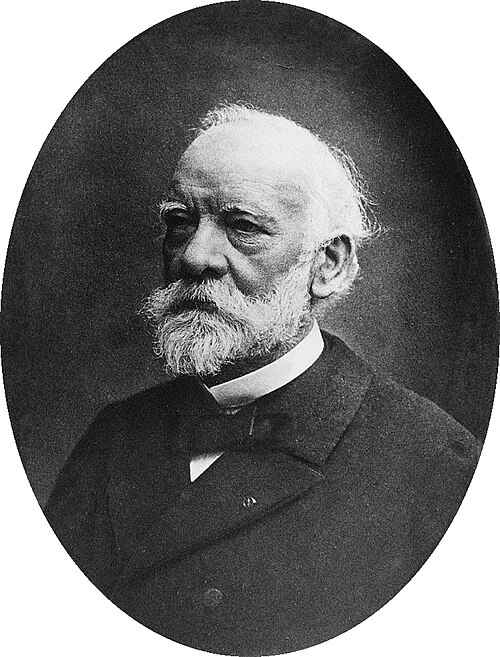
\includegraphics[width=\linewidth]{images/book3/friedel.jpg}
\end{minipage}\hspace{0.02\linewidth}%
\begin{minipage}[t]{0.18\linewidth}
\vspace{0pt}
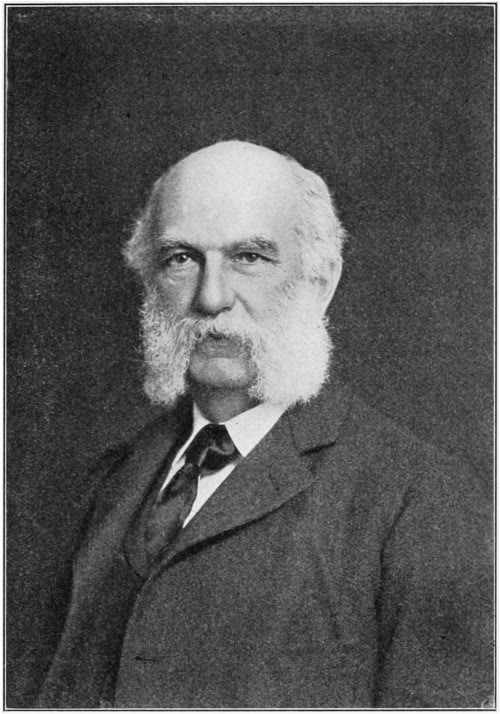
\includegraphics[width=\linewidth]{images/book3/crafts.jpg}
\end{minipage}\hfill
\begin{minipage}[t]{0.58\linewidth}
\vspace{0pt}
En 1877, Charles Friedel y James Mason Crafts, que trabajaban juntos en París, descubrieron que
el cloruro de aluminio hace reaccionar los halogenoalcanos y los cloruros de acilo con el benceno. Sus
reacciones se convirtieron en el método estándar para unir grupos carbonados a anillos \omterm{def:b2:huckel:aromatic}{aromáticos}, y la catálisis
por ácidos de Lewis que descubrieron llegó mucho más lejos. (Retratos: Friedel, década de 1890; Crafts, de
\textit{Popular Science Monthly}, 1900; dominio público, Wikimedia Commons.)
\end{minipage}
\end{history}

\begin{safety}{\ghs[5mm]{GHS02}\,\ghs[5mm]{GHS05}\,\ghs[5mm]{GHS06}\,\ghs[5mm]{GHS08}}
El benceno es cancerígeno y se sustituye por tolueno u otros \omterm{def:b2:aromatic-substitution:arene}{arenos} siempre que es posible.
Los ácidos nítrico y sulfúrico concentrados son corrosivos y la mezcla nitrante es fuertemente
oxidante; se enfría y el \omterm{def:b2:aromatic-substitution:arene}{areno} se añade lentamente, pues las nitraciones son \omterm{def:b2:reaction-enthalpy:exothermic}{exotérmicas}.
El bromo es muy tóxico y corrosivo; el cloruro de aluminio reacciona violentamente con el agua. Los nitroarenos
son tóxicos.
% ledger: ghs:benzene, ghs:toluene, ghs:HNO3, ghs:H2SO4, ghs:Br2, ghs:AlCl3, ghs:nitrotoluene-4
\end{safety}

\section{Ejercicios}

\begin{exercise}[$\star$]\label{exo:b2:aromatic-substitution:1}
Escríbase la formación del ion nitronio a partir del ácido nítrico y el ácido sulfúrico.
\end{exercise}

\begin{exercise}[$\star$]\label{exo:b2:aromatic-substitution:2}
Dense los productos principales de la bromación (\ce{Br2}, \ce{FeBr3}) del tolueno y del
nitrobenceno.
\end{exercise}

\begin{exercise}[$\star$]\label{exo:b2:aromatic-substitution:3}
Clasifíquense como activantes o desactivantes, orto/para o meta: \ce{-CH3}, \ce{-OH}, \ce{-Cl},
\ce{-NO2}, \ce{-COCH3}, \ce{-NHCOCH3}.
\end{exercise}

\begin{exercise}[$\star$]\label{exo:b2:aromatic-substitution:4}
Dese el producto del benceno con cloruro de etanoílo y cloruro de aluminio.
\end{exercise}

\begin{exercise}[$\star\star$]\label{exo:b2:aromatic-substitution:5}
El benceno y el 1-cloropropano con \ce{AlCl3} dan principalmente isopropilbenceno. Explíquese, y dese una
vía en dos etapas hacia el propilbenceno.
\end{exercise}

\begin{exercise}[$\star\star$]\label{exo:b2:aromatic-substitution:6}
El fenol decolora el agua de bromo de inmediato, sin catalizador, dando
2,4,6-tribromofenol. Explíquese.
\end{exercise}

\begin{exercise}[$\star\star$]\label{exo:b2:aromatic-substitution:7}
Dense síntesis del 3-bromonitrobenceno y del 4-bromonitrobenceno a partir del benceno.
\end{exercise}

\begin{exercise}[$\star\star$]\label{exo:b2:aromatic-substitution:8}
La anilina se nitra mal (oxidación, y producto meta), pero la acetanilida da principalmente
4-nitroacetanilida. Explíquense ambos hechos.
\end{exercise}

\begin{exercise}[$\star\star$]\label{exo:b2:aromatic-substitution:9}
Muéstrese cómo puede usarse un grupo ácido sulfónico para preparar 2-bromotolueno libre de su isómero para.
\end{exercise}

\begin{exercise}[$\star\star\star$]\label{exo:b2:aromatic-substitution:10}
¿Dónde se nitra el 4-metilanisol (4-metoxitolueno)? Explíquese con los dos
grupos orientadores.
\end{exercise}

\begin{exercise}[$\star\star\star$]\label{exo:b2:aromatic-substitution:11}
El 2,4,6-trinitrotolueno se obtiene por tres nitraciones sucesivas del tolueno, cada una en condiciones
más severas. Explíquese por qué.
\end{exercise}

\begin{exercise}[$\star\star\star$]\label{exo:b2:aromatic-substitution:12}
Propóngase una síntesis del ácido 4-nitrobenzoico a partir del tolueno, y otra del ácido 3-nitrobenzoico.
\end{exercise}

\section{Problema: nitrar el tolueno}

\begin{problem}[{Problema de fin de semana --- el ion nitronio y el mecanismo de la nitración, las
posiciones orto, meta y para del tolueno frente a la proporción estadística, la separación de los
isómeros y un balance de materia}]
\label{pb:b2:aromatic-substitution:1}
Datos: puntos de fusión: 2-nitrotolueno \qty{-10}{\degreeCelsius}, 3-nitrotolueno
\qty{16}{\degreeCelsius}, 4-nitrotolueno \qty{52}{\degreeCelsius}. Datos de una operación de ejercicio:
\qty{100}{g} de tolueno, \omterm{def:b2:continuous-reactors:conversion}{conversión} del 90~\%, distribución de isómeros 58~\% orto, 4~\% meta,
38~\% para. Masas molares (\unit{g/mol}): C 12.011, H 1.008, N 14.007, O 15.999.
% ledger: mp:2-nitrotoluene, mp:3-nitrotoluene, mp:4-nitrotoluene, aw:C, aw:H, aw:N, aw:O

\medskip
\noindent\textbf{Parte I --- El electrófilo y el mecanismo.}
\begin{enumerate}
  \item Escríbase la formación del ion nitronio.
  \item Dibújese su estructura de Lewis e indíquese su geometría.
  \item Escríbase el ataque del \ce{NO2+} al tolueno en para respecto al metilo.
  \item Dibújense las tres estructuras de resonancia del \omterm{def:b2:aromatic-substitution:seAr}{intermedio de Wheland} para.
  \item ¿Qué etapa es la determinante de la velocidad?
  \item ¿Qué retira el protón en la segunda etapa?
\end{enumerate}

\medskip
\noindent\textbf{Parte II --- Las tres posiciones.}
\begin{enumerate}[resume]
  \item ¿Cuántas posiciones orto, meta y para tiene el tolueno?
  \item ¿Qué proporción daría un ataque al azar?
  \item Dibújese el \omterm{def:b2:aromatic-substitution:seAr}{intermedio de Wheland} meta y explíquese por qué es el menos estabilizado.
  \item ¿Cómo estabiliza el grupo metilo los intermedios orto y para?
  \item Compárese la proporción observada con la estadística: ¿qué posiciones están favorecidas?
  \item Compárese el rendimiento por posición en orto (la mitad del porcentaje orto) y en para.
        Propóngase una razón para la diferencia.
  \item ¿Se nitra el tolueno más deprisa o más despacio que el benceno?
\end{enumerate}

\medskip
\noindent\textbf{Parte III --- Separación.}
\begin{enumerate}[resume]
  \item ¿Qué isómero es sólido a temperatura ambiente?
  \item Propóngase cómo aislarlo de la mezcla por enfriamiento.
  \item ¿Por qué la simetría favorece un punto de fusión alto?
  \item ¿Cómo podrían separarse después los isómeros orto y meta?
  \item ¿Por qué son difíciles de separar estos isómeros por destilación simple?
\end{enumerate}

\medskip
\noindent\textbf{Parte IV --- Balance de materia.}
\begin{enumerate}[resume]
  \item Calcúlense las masas molares del tolueno y del nitrotolueno.
  \item Calcúlense las cantidades de tolueno y de nitrotolueno formado.
  \item Calcúlense las masas de los tres isómeros.
  \item ¿Qué reacción posterior debe evitarse enfriando y no usando ácido en exceso?
  \item ¿Cómo se obtendría ácido 4-nitrobenzoico a partir del isómero para?
  \item Indíquese la masa de 4-nitrotolueno obtenida a partir de \qty{100}{g} de tolueno en esta operación.
\end{enumerate}
\end{problem}
